\section{Разработка кросс-платформенного приложения на React Native}
\label{sec:section-2}

\subsection{Постановка задачи}
В последние годы произошел резкий рост популярности мобильных устройств: более половины трафика в сети приходится именно на мобильный сегмент\cite{mobile-traffic-stats}. Формат мобильного приложения предоставляет пользователю непрерывный доступ к обучающим материалам и позволяет гибко распределять время, затрачиваемое на изучение иностранных языков. Кроме того, мобильные приложения позволяют легко поддерживать актуальность материала, вводить новые методики и автоматизировать процесс обучения. Учитывая данные преимущества, мы реализуем обучающую систему в виде мобильного приложения с использованием алгоритмов ML.

Целью приложения мы ставим предоставление всего необходимого функционала пользователю для планомерного расширения своего словарного запаса на иностранном языке, причем будем уделять внимание не только на текстовому и смысловому аспектам, но и фонетике, правильному произношению.

Определим ключевой функционал приложения, необходимый для достижения поставленной цели:
\begin{itemize}
	\item Появление новых слов для изучения должно происходить через регулярные интервалы и сопровождаться уведомлениями.
	\item Слова, изученные в прошлом, спустя некоторое время снова должны появиться для повторения.
	\item Подбор слов должен зависеть от выбранного уровня сложности и интересов пользователя.
	\item Слова должны сопровождаться фонетической транскрипцией, переводом и примерами использования.
	\item Необходимо реализовать возможность прослушивания эталонного произношения слова или фразы.
	\item Функция проверки произношения должна позволять автоматически оценить правильность речи студента и указать на возможные ошибки.
	\item Необходимо реализовать возможность пройти тест по уже изученным словам.
\end{itemize}

В последующих пунктах мы сфокусируемся на реализации перечисленных функций и рассмотрим необходимые для этого технические средства.

\subsection{Структура и интерфейс приложения}
Разработку интерфейсов будем производить с использованием Sketch. Sketch является мощным инструментом для дизайна и прототипирования пользовательских интерфейсов с богатым функционалом: работа с векторной графикой, возможность создания компонентов, настройка динамических макетов, поддержка библиотек компонентов и система плагинов.

Приложение состоит из двух вкладок: главная лента и панель управления. Основная лента состоит из карточек с изучаемыми словами и содержит всю историю изучаемых слов. Каждая карточка относится к одному слову или фразе и включает в себя слово, его перевод, несколько примеров использования и ссылку на упражнение по фонетике. При нажатии на слово вверху карточки или любое из предложений в примерах, воспроизводится синтезированная по соответствующему тексту речь. Другой тип карточек --- это карточки с напоминанием о словах, изученных в прошлом, такие карточки содержат сразу несколько слов и позволяют по нажатию перейти к месту в ленте, где слово появилось впервые. Такая концепция представлена на рисунке \ref{fig:word-cards}.

Лента пополняется карточками каждый раз, когда появляется новое слово, а сами карточки наполняются в течении дня: через равные интервалы времени пользователь получает уведомление с новым примером, который появился в ленте. Такой метод обучения позволяет с помощью регулярного повторения постепенно увеличивать словарный запас студента без дополнительных затрат времени.

\begin{figure}[h]
	\centering
	\begin{subfigure}{0.3\textwidth}
		\centering
		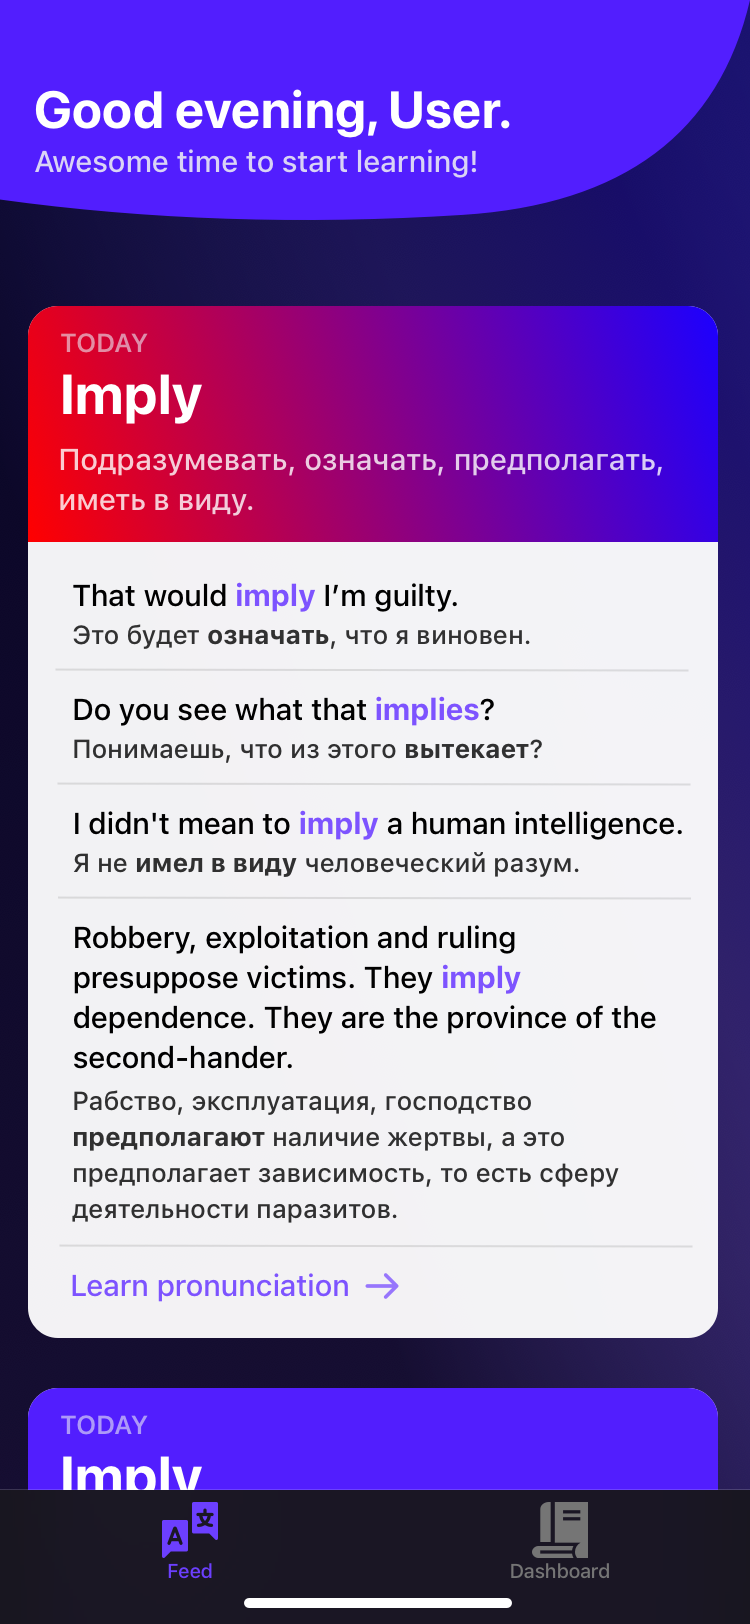
\includegraphics[width = \textwidth]{word-card}
%		\caption{Left figure}
%		\label{fig:left}
	\end{subfigure}
	\hspace{0.2\textwidth}
	\begin{subfigure}{0.3\textwidth}
		\centering
		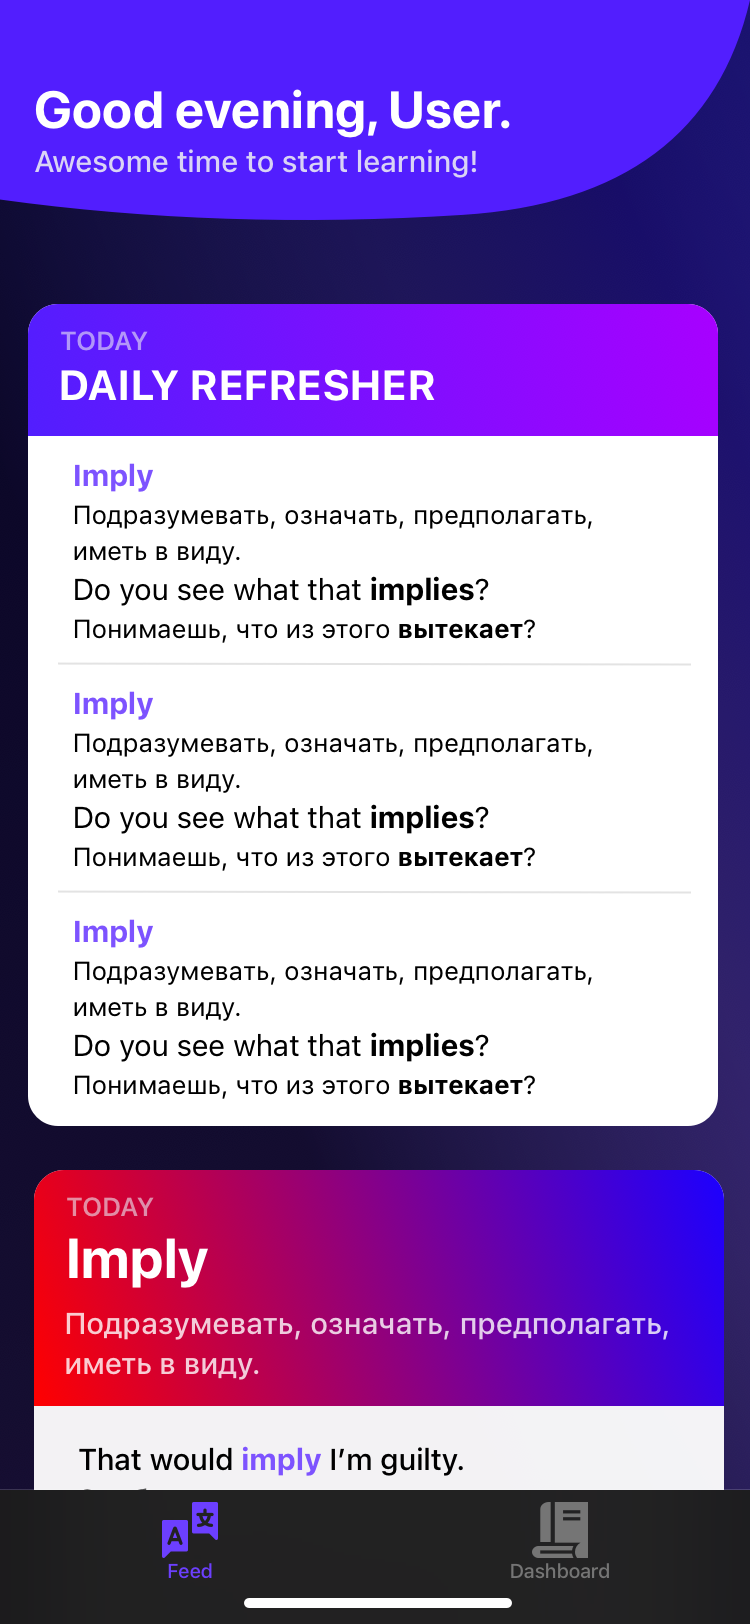
\includegraphics[width = \textwidth]{refresh-card}
%		\caption{Right figure}
%		\label{fig:right}
	\end{subfigure}
	%\hfill
	\caption{Внешний вид карточек основной ленты}
	\label{fig:word-cards}
\end{figure}

Экран панели управления содержит кнопки перехода к другим разделам и параметрам приложения: избранное, настройки, информация о программе, кнопки добавления новых слов и начала теста. Панель управления и некоторые из страниц, на которые можно с нее попасть, изображены на рисунке \ref{fig:dashboard}. На странице теста пользователь может проверить свои знания на случайном наборе изученных слов. В настройках представлены разнообразные параметры, включая уровень сложности, интересы и конфигурацию уведомлений. Уровень сложности и интересы студента, выбранные в настройках, влияют на то, какие слова будут появляться в ленте.

Страница фонетического упражнения позволяет пользователю прослушать эталонное произношение и проверить свое собственное на примере отдельных слов или целых предложений. Результат проверки содержит ключевые характеристики речи: общее качество произношения, беглость, пропущенные и лишние слова, после чего приводится анализ произношения каждого слова по фонемам. Визуальное представление этой страницы приводится на рисунке \ref{fig:pronunciation-check}. Подробный анализ произношения студента по фонемам позволяет давать качественную обратную связь, указывая на точные места ошибок в речи.

\begin{figure}[H]
	\centering
	\begin{subfigure}{0.3\textwidth}
		\centering
		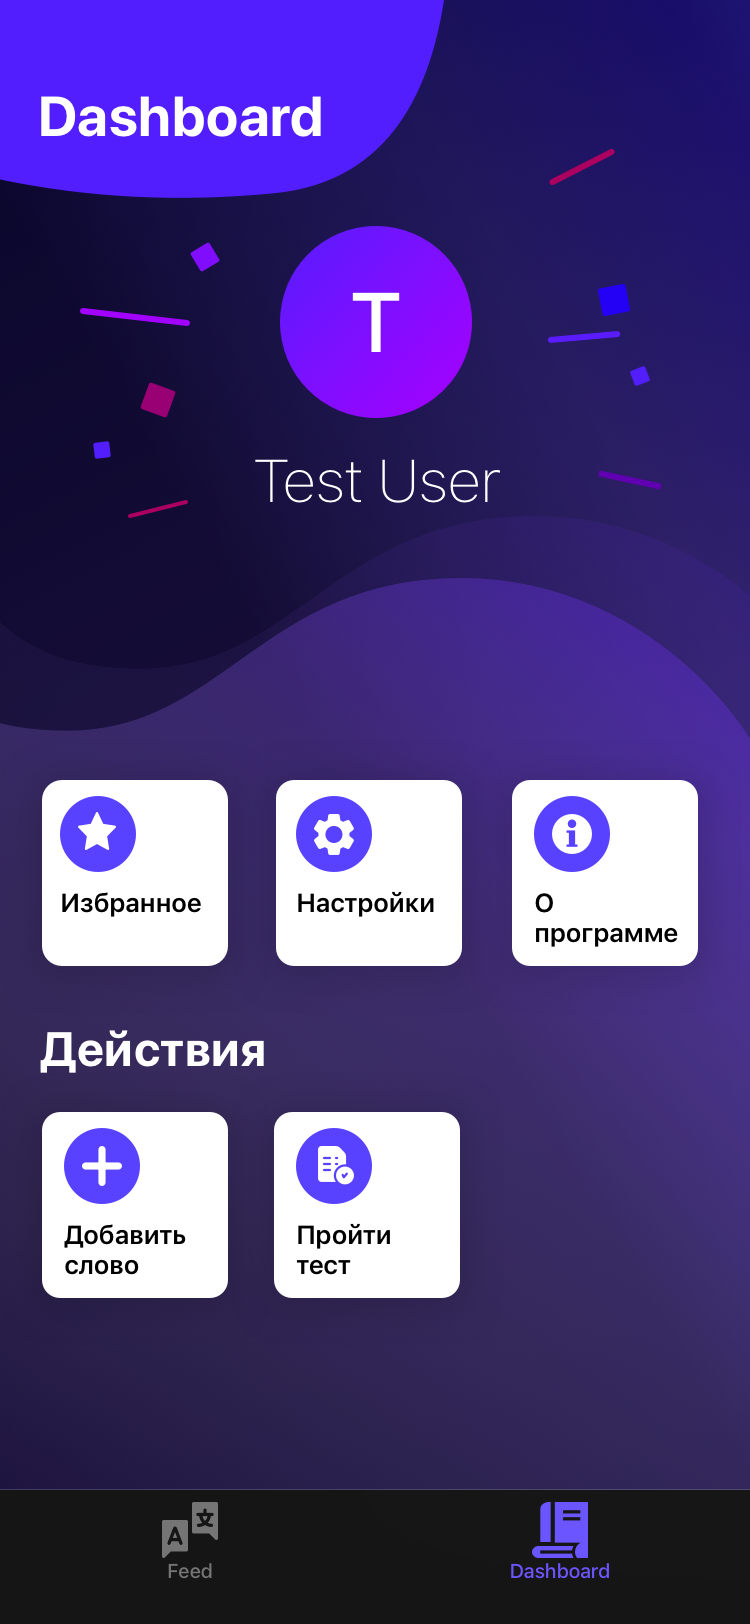
\includegraphics[width = \textwidth]{dashboard}
	\end{subfigure}
%	\hspace{0.05\textwidth}
	\begin{subfigure}{0.3\textwidth}
		\centering
		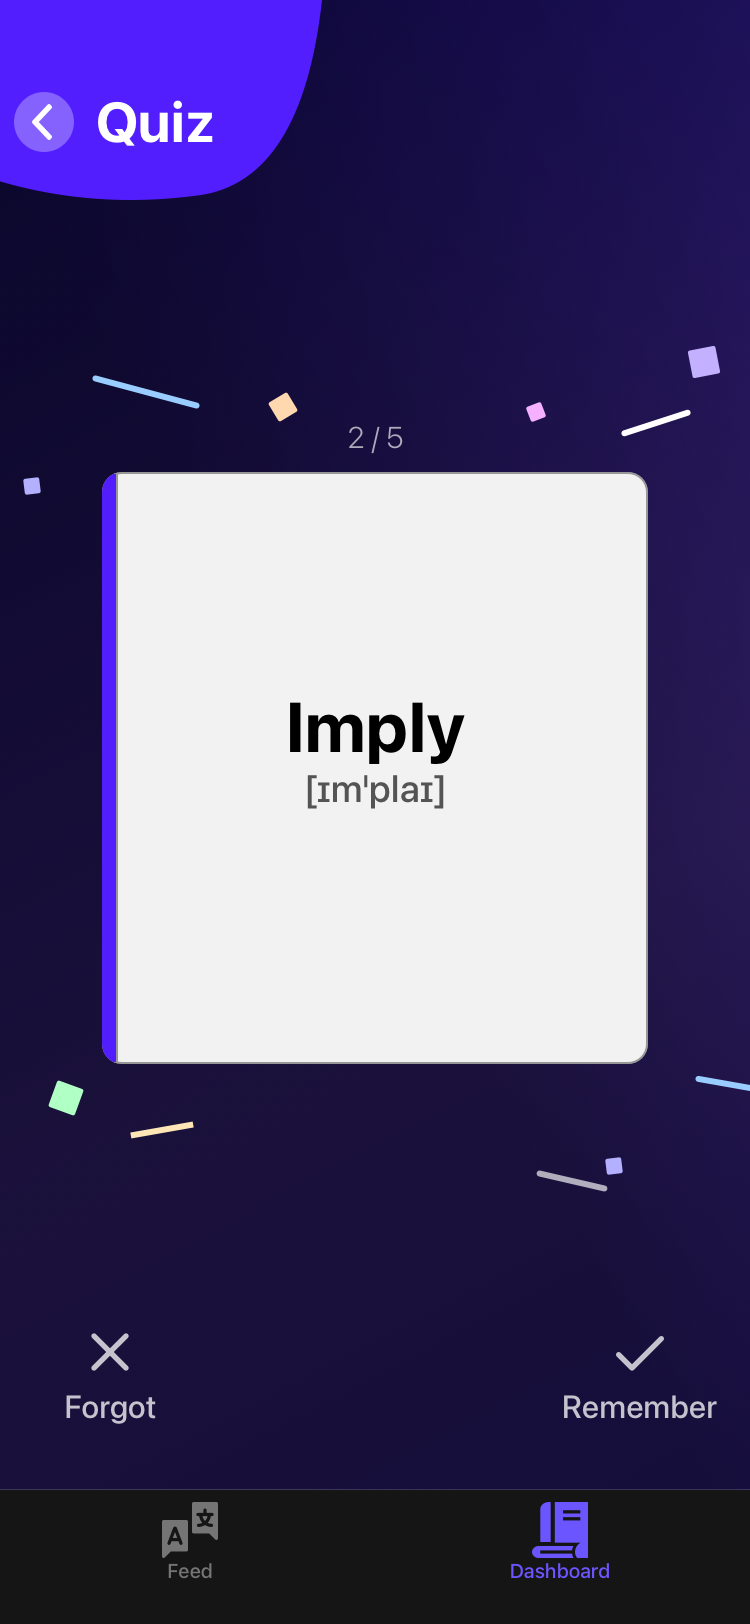
\includegraphics[width = \textwidth]{quiz}
	\end{subfigure}
%	\hspace{0.05\textwidth}
	\begin{subfigure}{0.3\textwidth}
		\centering
		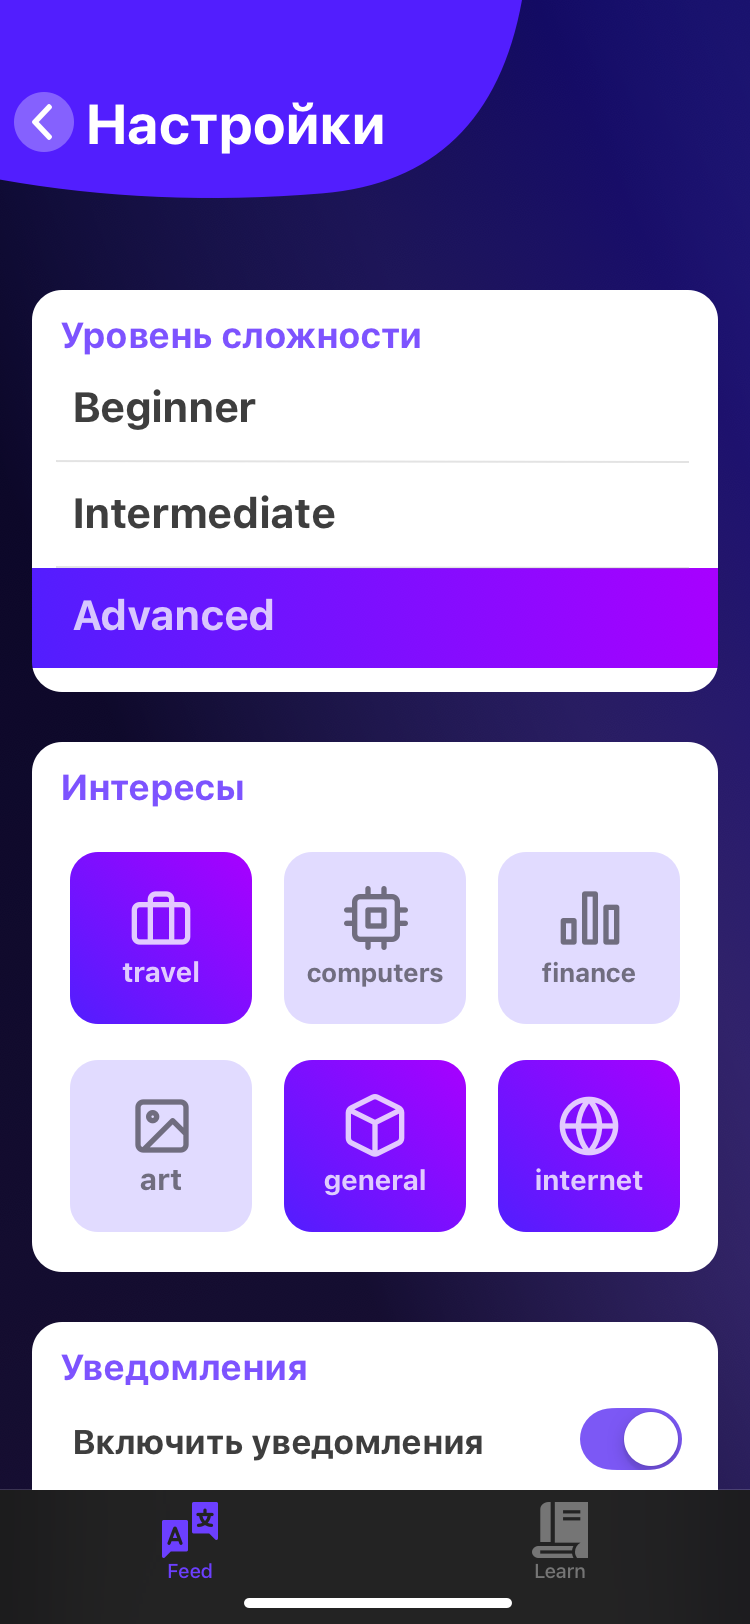
\includegraphics[width = \textwidth]{settings}
	\end{subfigure}
	\caption{Интерфейс панели управления, теста и настроек}
	\label{fig:dashboard}
\end{figure}

\begin{figure}[H]
	\centering
	\begin{subfigure}{0.3\textwidth}
		\centering
		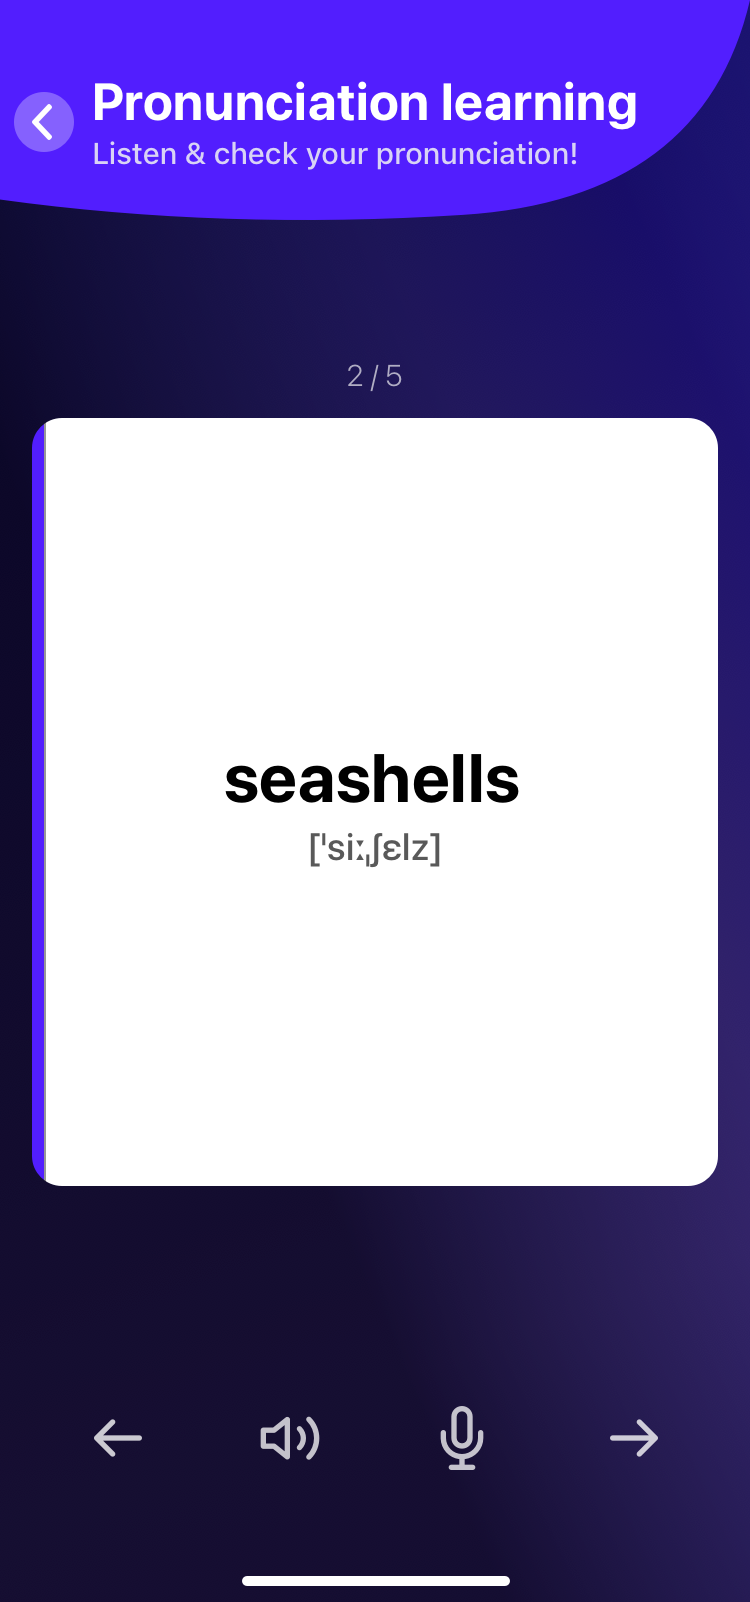
\includegraphics[width = \textwidth]{pronunciation-check}
	\end{subfigure}
	\hspace{0.2\textwidth}
	\begin{subfigure}{0.3\textwidth}
		\centering
		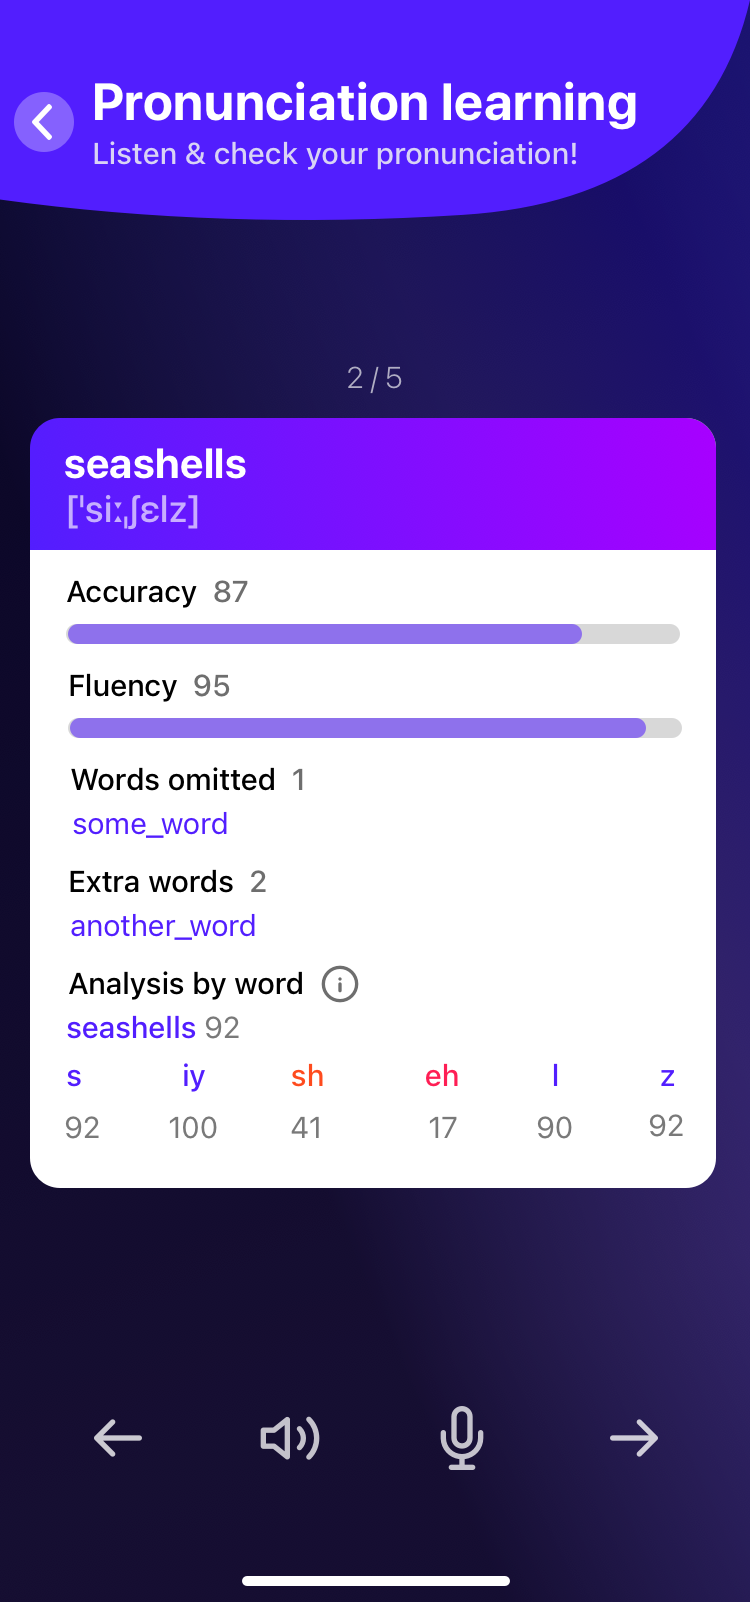
\includegraphics[width = \textwidth]{pronunciation-results}
	\end{subfigure}
	\caption{Страница проверки и анализа произношения}
	\label{fig:pronunciation-check}
\end{figure}

\subsection{Программная реализация приложения}
В качестве стека технологий для реализации кросс-платформенного приложения был выбран React Native и TypeScript. 

Такой выбор обусловлен следующими преимуществами этих технологий:
\begin{itemize}
	\item React Native позволяет разрабатывать нативные приложения с использованием React и JavaScript, иметь единую кодовую базу и набор компонентов под все платформы. В отличие от таких продуктов, как Ionic или Apache Cordova, для отображения интерфейса React Native использует именно нативные компоненты, а не WebView. Это достигается с помощью архитектуры, состоящей из трех компонентов: JavaScript VM --- RN bridge --- Native API.
	\item Архитектура приложения, основанная на компонентах, и построенная на концепциях React.
	\item Использование JavaScript открывает доступ к богатому разнообразию пакетов на npm --- их насчитывается свыше 1.3 миллионов.
	\item Удобство разработки с использованием hot--reloading, применения изменений в реальном времени.
	\item Возможность обновлять приложения over--the--air, то есть загружать новые версии в фоновом режиме и применять их на следующем запуске, вместо выпуска обновлений через магазин приложений платформы и ожидания подтверждения со стороны Apple или Android.
	\item TypeScript добавляет в JavaScript статическую типизацию, что позволяет обнаруживать широкий класс ошибок уже на этапе сборки. Кроме того, код на TypeScript отлично интегрируется с IDE при разработке, а также облегчает рефакторинг и отладку.
\end{itemize}

Для краткости мы не будем приводить здесь весь исходный код приложения, а представим верхне--уровневый обзор архитектуры проекта и наиболее важных технических деталей.
Структура проекта определяется разделением сущностей по своему типу: компоненты, ресурсы, react--хуки, файлы связанные с навигацией, и различные экраны. % Детальнее со структурой приложения можно ознакомиться на рисунке \ref{label}.

Для навигации используется пакет react-navigation, позволяющий быстро создавать гибкие сценарии перемещения между различными частями приложения при помощи расширяемых компонентов. Компоненты, используемые в данном пакете, автоматически адаптируются под целевую платформу и имеют привычное для пользователя поведение, включая анимации и жесты. Пример того, как в нашем проекте определяется навигация между двумя вкладками, приводится на листинге \ref{lst:react-navigation}.
\begin{lstlisting}[basicstyle=\fontsize{11}{11}\selectfont,tabsize=4,breaklines=true,caption={Навигация с использованием вкладок.},captionpos=b,label={lst:react-navigation}]
function BottomTabNavigator() {
  const BottomTab = createBottomTabNavigator<BottomTabParamList>();
  const colorScheme = useColorScheme();

  return (
    <BottomTab.Navigator
      initialRouteName="Feed"
      tabBarOptions={{
          activeTintColor: Colors[colorScheme].tint,
          style: tabBarStyle,
      }}>
      <BottomTab.Screen
        name="Feed"
        component={FeedScreen}
      />
      <BottomTab.Screen
        name="Dashboard"
        component={DashboardScreen}
      />
    </BottomTab.Navigator>
  );
}
\end{lstlisting}

Для отображения ленты с карточками на основной странице мы используем компонент FlatList, позволяющий отрисовывать длинные списки элементов не теряя производительности на разных платформах. В листинге \ref{lst:feed-screen} приводится слегка упрощенная версия устройства главной ленты.
\begin{lstlisting}[basicstyle=\fontsize{11}{11}\selectfont,tabsize=4,breaklines=true,caption={Структура главной ленты с карточками.},captionpos=b,label={lst:feed-screen}]
// WordCard.tsx
function WordCard(props) {
  let { examples, style } = props;
  _.defaultsDeep(style, defaultStyle);
  // ...
  return (
    <View style={style.card}>
      // ...
    </View>
  );
}

// FeedScreen.tsx
// ...
<FlatList
  ListHeaderComponent={<Header/>}
  ListHeaderComponentStyle={flatListHeaderStyles}
  data={feedItems}
  renderItem={() => <WordCard /*...*/ />}
/>
\end{lstlisting}

При реализации панели управления был разработан ряд кастомных компонентов, для панелей кнопок используется ScrollView, а фоновое изображение отрисовывается при помощи svg. Схема реализации макета панели управления приводится в листинге \ref{lst:dashboard-screen}.
\begin{lstlisting}[basicstyle=\fontsize{11}{11}\selectfont,tabsize=4,breaklines=true,caption={Структура страницы панели управления.},captionpos=b,label={lst:dashboard-screen}]
<LinearGradient>
  <WaveBackground /* ... *//>
  <Header /* ... *//>
  <View style={styles.userContainer}>
    <ProfilePicture /* ... *//>
    <Text style={styles.userName}>/* ... */</Text>
  </View>
  <View style={styles.actionsContainer}>
    <Text style={styles.actionsSectionHeader}>/* ... */</Text>
    <ScrollView horizontal={true} style={styles.actionsButtonsContainer}>
      { mainButtons }
    </ScrollView>

    <Text style={styles.actionsSectionHeader}>/* ... */</Text>
    <ScrollView horizontal={true} style={styles.actionsButtonsContainer}>
      { actionButtons }
    </ScrollView>
</View>
</LinearGradient>
\end{lstlisting}

Для хранения и получения данных мы будем использовать Firestore от Firebase, интерфейс к которому предоставляется пакетами firebase и @react-native-firebase/app. Firestore --- это гибкая и расширяемая облачная NoSQL база данных, обладающая богатым функционалом: возможность синхронизации данных между сервером и несколькими устройствами в реальном времени, поддержка кэширования на случай отсутствия подключения и удобное API для запросов. В сочетании с другими сервисами Firebase, Firestore позволяет значительно ускорить разработку как прототипов приложений, так и финальных версий, предназначенных для конечного пользователя. Рассмотрим пример использования Firestore в контексте нашего приложения на листинге \ref{lst:firestore-usage}.

\begin{lstlisting}[basicstyle=\fontsize{11}{11}\selectfont,tabsize=4,breaklines=true,caption={Использования Firestore для получения данных карточек главной ленты.},captionpos=b,label={lst:firestore-usage}]
import firebase from 'firebase';
import 'firebase/firestore';

firebase.initializeApp(/* config */);
const db = firebase.firestore();

const words = db.collection('words').get().then(wordDocs => {
  wordDocs.forEach(wordDoc => console.log(`${wordDoc.id} - ${wordDoc.data()}`));
});

\end{lstlisting}


В качестве системы контроля версий используется git, с хостингом в репозитории на bitbucket. Даже бесплатная версия bitbucket предоставляет широкий спектр возможностей. Так, например, CI/CD пайплайны позволяют автоматизировать процесс тестирования, сборки и публикации пакетов. Простой файл конфигурации представлен на листинге \ref{lst:bitbucket-pipeline}. Такой пайплайн позволяет запускать линтеры и тесты в PR--ах и автоматически публиковать изменения при влитии в master.

\begin{lstlisting}[basicstyle=\fontsize{11}{11}\selectfont,tabsize=4,breaklines=true,caption={Пример конфигурации сборочного конвейера bitbucket.},captionpos=b,label={lst:bitbucket-pipeline}]
image: node:16
pipelines:
  default:
    - step:
        script:
          - npm run lint
          - npm run test
  branches:
    master:
      - step:
          deployment: production
          script:
            - npm run test
            - ./deploy.sh production
\end{lstlisting}

Другими инструментами разработки, которые используются в проекте, являются ESLint и Prettier. ESLint с конфигурацией от airbnb позволяет быстро обнаруживать проблемные места в коде и ввести определенный набор правил оформления javascript/typescript кода. Prettier же отлично справляется с задачей форматирования файлов в самых разных форматах, включая typescript, json и yaml файлы. Таким образом в кодовой базе всегда поддерживается единый стандарт написания кода.

\subsection{Вывод по разделу}
В данном разделе мы рассмотрели процесс разработки фронтенда приложения от начальных стадий до завершающих.

Сначала мы формализовали требования, предъявляемые к приложению --- регулярное появление слов в ленте, возможность проверки произношения и анализа ошибок, функция проверки пройденного материала, присутствие настроек по интересам и уровню сложности.

Далее была разработана структура приложения и макеты всех основных элементов интерфейса с использованием Sketch. В ходе проектирования было создано свыше 30 вариаций дизайна интерфейса и десятки компонентов, из числа которых в работе представлена выборка наиболее удачных.

Наконец, мы рассмотрели процесс разработки приложения с использованием технологий React Native, TypeScript и Firebase. Мы коснулись аргументации выбора такого стека библиотек, а также основных технических деталей реализации, включая инфраструктурные аспекты --- линтинг, сборка и настройка CI/CD в репозитории. Мы не приводим слишком большого количества кода в данном разделе из соображений удобства --- код хранится в системе контроля версий.

Следующий раздел будет посвящен ещё одному крупному фрагменту нашего сервиса --- backend инфраструктуре.